
\section{Theorie}
\label{sec:Theorie}

\subsection{Spin $s$, Bahndrehimpuls $l$ und magnetisches Moment $\mu$}

Jedes Elektron in der Hülle eines Atoms besitzt einen quantisierten Bahndrehimpuls $\vec{l}$ und Spin $\vec{s}$ mit den Beträgen:
\begin{align*}
	|\vec{l}|= \hbar \sqrt{l(l+1)}&\text{ mit } l=0,1,\hdots,n-1\\
	|\vec{s}|= \hbar \sqrt{s(s+1)}&\text{ mit } s=\frac{1}{2}\text{.}
\end{align*}
\noindent Mit dem Bohrschen Magneton $\mu_.B=\frac{e_0 \hbar}{2 m_0}$, mit Elektronenladung und -masse $e_.0$ und $m_.0$ und dem reduzierten Planckschen Wirkungsquantum $\hbar$, und dem gyromagnetischen Verhältnis des Elektrons $g_.e\approx 2$, lassen sich die jeweiligen magnetischen Momente berechnen zu
\begin{gather*}
	\vec{\mu}_l=-\mu_.{B} \sqrt{l(l+1)} \vec{e}_.l, \\
	\vec{\mu}_s=- g_.{s} \mu_.{B} \sqrt{s(s+1)} \vec{e}_.s\text{.}
\end{gather*}
Dabei sind $\vec{e}_.l$ und $\vec{e}_.s$ die Einheitsvektoren von Bahndrehimpuls und Spin. Der Unterschied der beiden Momente um das gyromagnetischen Verhältnis wird als magnetomechanische Anomalie bezeichnet.


\subsection{$LS$- und $jj$-Kopplung}

Die Kopplung von Spin und Bahndrehimpuls variiert stark mit der Kernladungszahl $Z$. Es können jedoch zwei Grenzfälle für leichte bzw. schwere Kerne behandelt werden.\\
Für geringe $Z$ ist die $LS$-Kopplung dominant. Sie tritt auf, wenn die Kopplung zwischen Spinmoment und Bahndrehimpulsmoment desselben Teilchens klein ist gegenüber den Kopplungen der Spinmomente und Bahndrehimpulsmomente zwischen den Hüllenelektronen. In diesem Fall koppeln diese zu einem Gesamtdrehimpuls und Gesamtspin 
\begin{align*}
\vec{L} &= \sum \vec{l}_.i \text { und }\\
\vec{S} &= \sum \vec{s}_.i,
\end{align*}
wobei nur die Elektronen in nicht abgeschlossenen Schalen beitragen, da sich Spins und Bahndrehimpulse in jeder vollen Schale gegenseitig aufheben.
Der Gesamtdrehimpuls ergibt sich damit zu
\[
\vec{J}=\vec{L}+\vec{S}
\]
und das gesamte magnetische Moment zu
\begin{equation}
\vec{\mu}_.J=\vec{\mu}_.L+\vec{\mu}_.S \label{eq:mu_ges}
\end{equation}
Dadurch entstehen Feinstrukturaufspaltungen die sich nur in der Quantenzahl $J$ unterscheiden und deren Energieniveaus um
\begin{align*}
\Delta E_.{LS} &= c \vec{L}\cdot\vec{S}\\
&= c \left[J(J+1)-L(L+1)-S(S+1)\right]\hbar^2
\end{align*}
verschoben sind, mit der zustandsabhängigen Konstanten $c$. Da diese Korrektur klein gegenüber den Hauptenergieniveaus ist lassen sich im Spektrum nicht überlagerte Multipletts beobachten.
Der zweite Grenzfall für schwere Kerne wird $jj$-Kopplung genannt. Hierbei tragen die Kopplungen von $\vec{s}$ und $\vec{l}$ der einzelnen Elektronen stärker bei als die Kopplungen untereinander, sodass sich einzelne Gesamtdrehimpulse der Elektronen bilden:
\[
\vec{j}_.i=\vec{l}_.i+\vec{s}_.i
\]
Diese bilden gemeinsam den Gesamtdrehimpuls
\[
\vec{J}=\sum_.i \vec{j}_.i
\]
Die Spektrallinien der aufgespaltenen Zustände überlagern sich in diesem Fall.
Für das Spektrum des in diesem Versuch verwendeten Cadmium liegt eine intermediäre Kopplung vor die eine Überlagerung dieser beiden Grenzfälle darstellt.

\subsection{Auswahlregeln für Zustandsänderungen}

Zwischen zwei Energieeigenzuständen sind verschiedene Übergänge möglich, jedoch gibt es verbotene Prozesse, die stark unterdrückt sind. Aus der Lösung der zeitabhängigen Schrödingergleichung ergibt sich eine Bedingung für die Änderung der Quantenzahl $m$ beim Übergang:
\begin{equation}
\Delta m = 0 \lor \pm 1 \label{eq:regeln}
\end{equation}
$\Delta m = 0$ entspricht dabei der linear polarisierten $\pi$-Komponente und $\Delta m = \pm 1$ der zirkular polarisierten $\sigma$-Komponente der emittierten Strahlung.
Der $\sigma$-Anteil besitzt demnach eine longitudinale und eine transversale Komponente, wobei die transversale Komponente senkrecht auf der transversalen Komponente des $\pi$-Anteils steht.

\subsection{Normaler und Anomaler Zeeman-Effekt, Paschen-Back-Effekt}

Bei der Aufspaltung der Zustände im äußeren Magnetfeld sind nur die Anteile des magnetischen Moments aus Gleichung \eqref{eq:mu_ges} von Belang, die parallel zu $\vec{B}$ ausgerichtet sind, da die senkrechten im zeitlichen Mittel verschwinden.
Der Betrag des magnetischen Moments berechnet sich dabei nach:
\[
\begin{split}
|\vec{\mu}_.J|&=\mu_.B \sqrt{J(J+1)} \cdot \frac{(1+g_.e) J (J+1) + (g_.e-1)\{S(S+1)-L(L+1)\}}{2 J (J+1)}\\
&= \mu_.B\cdot g_.J \cdot\sqrt{J(J+1)},
\end{split}
\]
Dabei wird $g_.J$ als Landé-Faktor bezeichnet. Auf Grund des Phänomens der Richtungsquantelung kann das magnetische Moment nur Richtungen annehmen, bei welchen die Komponente $\mu_.{J,||}$ entlang der Feldlinien ein ganzes Vielfaches von $\mu_.B \cdot g_.J$ ist und somit gilt:
\[
\mu_.{J, ||}=-\mu_.B g_.J \cdot m \text{ mit } m=-J,-J+1,\hdots, J
\]
Wegen der Begrenzung für $m$, gibt es somit $(2J+1)$ mögliche Zustände.
Die Energiekorrekturen dieser Zustände ergeben sich nach
\[
\Delta E_.m = = \mu_.B g_.J B \cdot m,
\]
sodass die Aufspaltung proportional zur Stärke des Magnetfeldes ist.
Zwischen den Zuständen sind nun allgemein Übergänge unter Abstrahlung eines Photons mit der Energie
\begin{equation*} 
	\begin{split}
	E_\gamma &= \Delta E = E_.2-E_.1 \\
	&=\{g_.{J_.2} \cdot m_.2-g_.{J_.1} \cdot m_1 \} \mu_.B B  + E_.0\\
	&=E_.{Auf}+E_.0
	\end{split}
\end{equation*}
möglich.
Dabei ist $E_.0$ die Emissionsenergie eines Photons, wenn keine Aufspaltung vorliegt und $E_.{Auf}$ die Energiedifferenz zwischen den aufgespaltenen Niveaus ist.
Für den normalen Zeeman-Effekt gilt $g_.{J_.i}=1$ und damit
\begin{equation}
E_.{\gamma,n} = \mu_B B \cdot \Delta m + E_.0
\end{equation}
Auf Grund der Auswahlregeln ($\Delta m = \pm 1$) werden somit nur zwei zusätzliche Linien im Übergangsspektrum erzeugt.
Beim anomalen Zeeman-Effekt (mit Spin) kommt es hingegen zu einer komplizierteren Aufspaltung, die allerdings nur für geringe Magnetfeldstärken und damit geringe Abstände der Multiplettkomponenten zu beobachten ist.
Für stärkere $\vec{B}$-Felder kommt es zum Paschen-Back-Effekt, der dazu führt das wieder nur das Zustandstriplett des normalen Zeeman-Effekts sichtbar ist.


\subsection{Die Lummer-Gehrcke-Platte}
In Abbildung \ref{fig:LGP} ist der Querschnitt einer Lummer-Gehrcke-Platte zu sehen.
Sie kann dazu verwendet werden eintreffendes Licht mit hoher Auflösung in die Spektrallinien zu zerlegen.
Das Licht trifft auf ein Prisma und wird so auf die planparallele Platte gelenkt. Der Winkel der auftreffen liegt dabei nahe dem kritischen Winkel, sodass nach Eintreten in die Platte, ein Großteil des Lichts im Glas reflektiert, jedoch ein kleiner Anteil bei jedem Auftreffen auf die Oberflächen transmittiert. Diese austretenden Strahlen bilden ein Interferenzmuster, welches aufgenommen werden kann.
Besteht der einfallende Lichtstrahl nicht aus Licht einer Wellenlänge $\lambda$, sondern zwei leicht um $\delta \lambda$ zu $\lambda$ verschiedene Wellenlängen, dürfen diese sich, mit der Dicke der Platte $d$ und dem Brechungsindex in der Platte $n$, maximal um
\begin{equation}
	\Delta\lambda_.{D} = \frac{\lambda^2}{2 \cdot d} \cdot \sqrt{\frac{1}{n^2-1}} \label{eq:disGebiet}
\end{equation}
unterscheiden, damit sich die Interferenzbilder nicht überlagern.
Das Auflösungsvermögen lässt sich mit der Länge der Lummer-Gehrcke-Platte $L$ berechnen zu
\begin{equation}
	A = \frac{\lambda}{\Delta\lambda} = \frac{L}{\lambda} \cdot \left(n^2-1\right), \label{eq:Aufloesung}
\end{equation}
Die Verschiebung der Wellenlängen um $\delta \lambda$ durch den Zeeman-Effekt macht sich im Interferenzbild durch eine Aufspaltung der Maxima in um $\delta s $ verschobene Maxima bemerkbar. Aus der Verschiebung $\delta s$ lässt sich, mit dem Abstand $\Delta s$ vom zugehörigen nicht aufgespaltenen Maxima zum Maxima nächst niedrigerer Ordnung, die Verschiebung der Wellenlänge $\delta \lambda$ berechnen zu
\begin{equation}
\delta \lambda = \frac{\delta s}{\Delta s} \Delta\lambda_\text{D} \label{eq:deltaLambda}
\end{equation}
und mit der Lichtgeschwindigkeit $c$ die Energieaufspaltung bestimmen:
\begin{equation}
E_.{Auf}=\frac{h c}{\lambda^2} \cdot (2\delta \lambda)\text{.} \label{eq:EaufExp}
\end{equation}
Ebenso ergibt sich damit für den Landé-Faktor
\begin{equation}
g_.{j}=\frac{h c}{\lambda^2 \cdot \mu_\text{B} B} \cdot (2\delta \lambda)\text{.} \label{eq:exgj}
\end{equation}
\begin{figure}
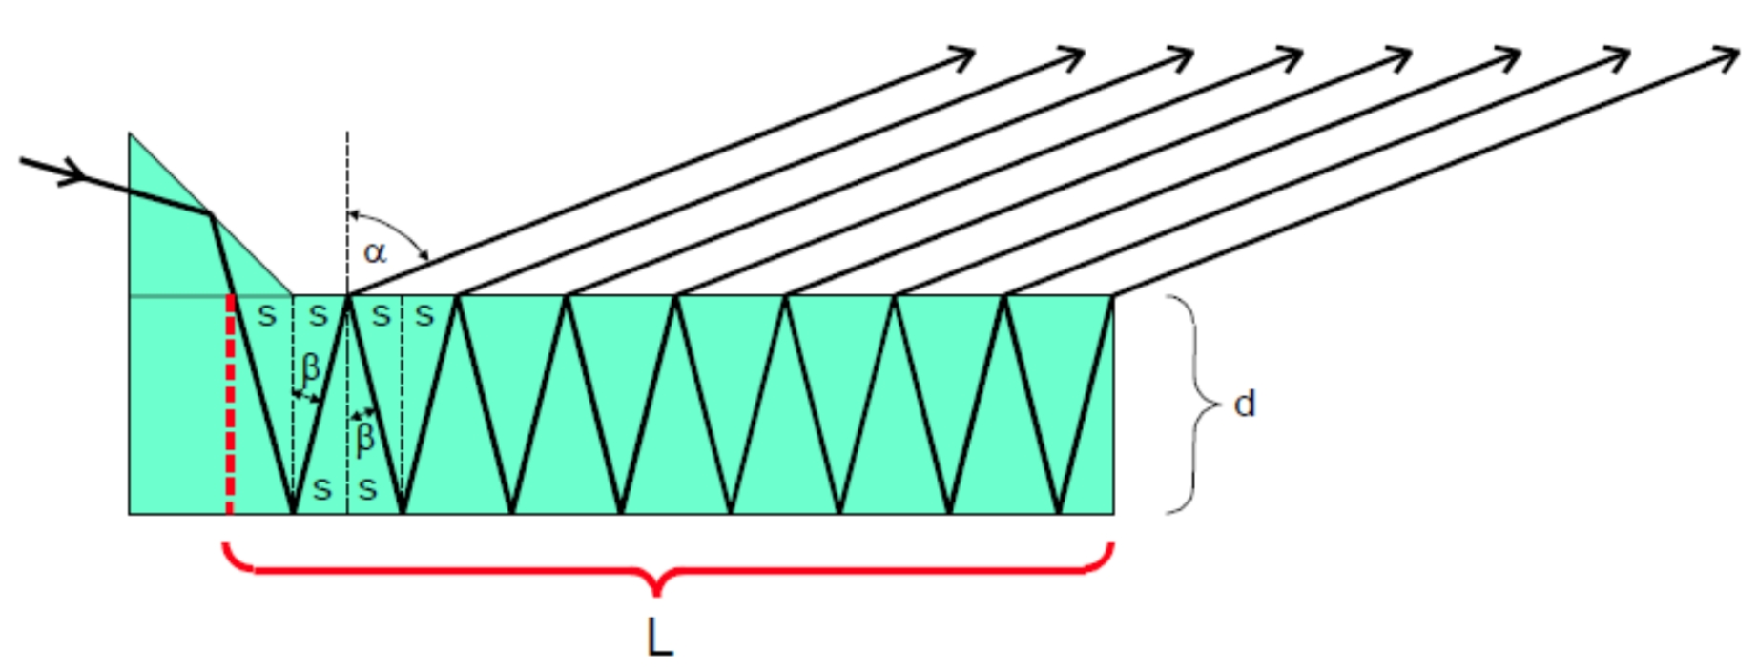
\includegraphics[width=0.8\textwidth]{content/images/LGP.pdf}
\caption{Schematische Darstellung des Querschnitts einer Lummer-Gehrcke-Platte.\cite{V27}}
\end{figure}
%◘